\documentclass[hidelinks,12pt,a4paper]{article}
\usepackage[italian]{babel}
\usepackage[utf8]{inputenc}
\usepackage{fourier} 

% Images
\usepackage{graphicx}
\usepackage{caption}
\usepackage{subcaption}
\usepackage{float}
\graphicspath{ {../Images} }

% Stop hyphenation
\usepackage[none]{hyphenat}

% To draw images
\usepackage{tikz}

% To generate jigsaw
\usepackage{jigsaw}

% Adjust paragraph.
\usepackage{changepage}
\usepackage{geometry}

% License
\usepackage[
type={CC},
modifier={by-nc-sa},
version={4.0},
]{doclicense}

\begin{document}
	
	\title{\textbf{\centering{Laboratorio creativo per bambini}\\Puzzle opere d'arte}}
	\author{Alice Balestieri\\Francesco Rombaldoni}
	\date{}
	
	\maketitle
	\newpage
	
	\tableofcontents
	\newpage
	
	\section{Come giocare}
	\begin{center}
		\textbf{Le regole sono rivolte agli operatori.}
	\end{center}
	
	\subsection{Variante 1}
	Dopo aver ritagliato i vari puzzle, mischiare i vari pezzi di tutti i puzzle ritagliati (per esempio mettendoli in una scatola per poi scuoterla), per poi disporli casualmente su di un tavolo. I bambini dovranno risolvere i vari puzzle riconoscendo i vari pezzi delle opere.\\
	Quando i bambini hanno finito di risolvere i puzzle, domandarli se si ricordano i nomi delle opere che hanno ricomposto.
	
	\subsection{Variante 2}
	Dopo aver ritagliato i vari puzzle, mischiare i vari pezzi di tutti i puzzle ritagliati (per esempio mettendoli in una scatola per poi scuoterla), per poi disporli casualmente al centro di un tavolo. Dividere i bambini in squadre da massimo tre elementi, successivamente assegnare ad ogni squadra due opere prese dalla lista delle opere trasformate in puzzle. I bambini dovranno cercare i vari pezzi dell'opera che devono ricomporre per poi risolvere i puzzle sui bordi del tavolo (queste due azioni possono essere fatte simultaneamente dai vari elementi del gruppo).
	
	\section{Lista delle opere trasformate in puzzle}
	\begin{itemize}
		\item Mengaroni Ferruccio - Medusa
		\item Bellini Giovanni - Incoronazione della Vergine
		\item Vitale da Bologna - Sant'Ambrogio in trono
		\item Desani Pietro - Rebecca ed Eleazar
		\item Leda e il Cigno (Giove) di fattura ad opera di Giovanni Antonio Garella
		\item Vedute di Roma
		\item Orologio notturno
		\item Scacciani Antonio - Vassoio - Rosa
		\item Milani Aureliano - Mercato
		\item Berentz Christian - Fiori e frutta con bicchieri di cristallo
		\item Gianlisi Antonio Junior - Trompe l'oeil con sonetto in onore di Eugenio di Savoia e mensola con oggetti
		\item Gianlisi Antonio Junior - Trompe l'oeil con paesaggio forbici e mensola con oggetti
		\item Realfonzo Tommaso - Natura morta con dolci frutta uova e formaggi
		\item Gessi Giovan Francesco - Morte di Adone
	\end{itemize}

	\section{Puzzle}

	\newgeometry{top=15mm, bottom=15mm}
	\begin{adjustwidth}{-30mm}{-30mm}
	
	% Start inserting images (used images formats from "Coloring_Artworks")
	
			\begin{minipage}{\linewidth}
			\centering
		
			\begin{tikzpicture}
			%	\clip (0,0) rectangle (6,4);
				\node at (0,0) {%
					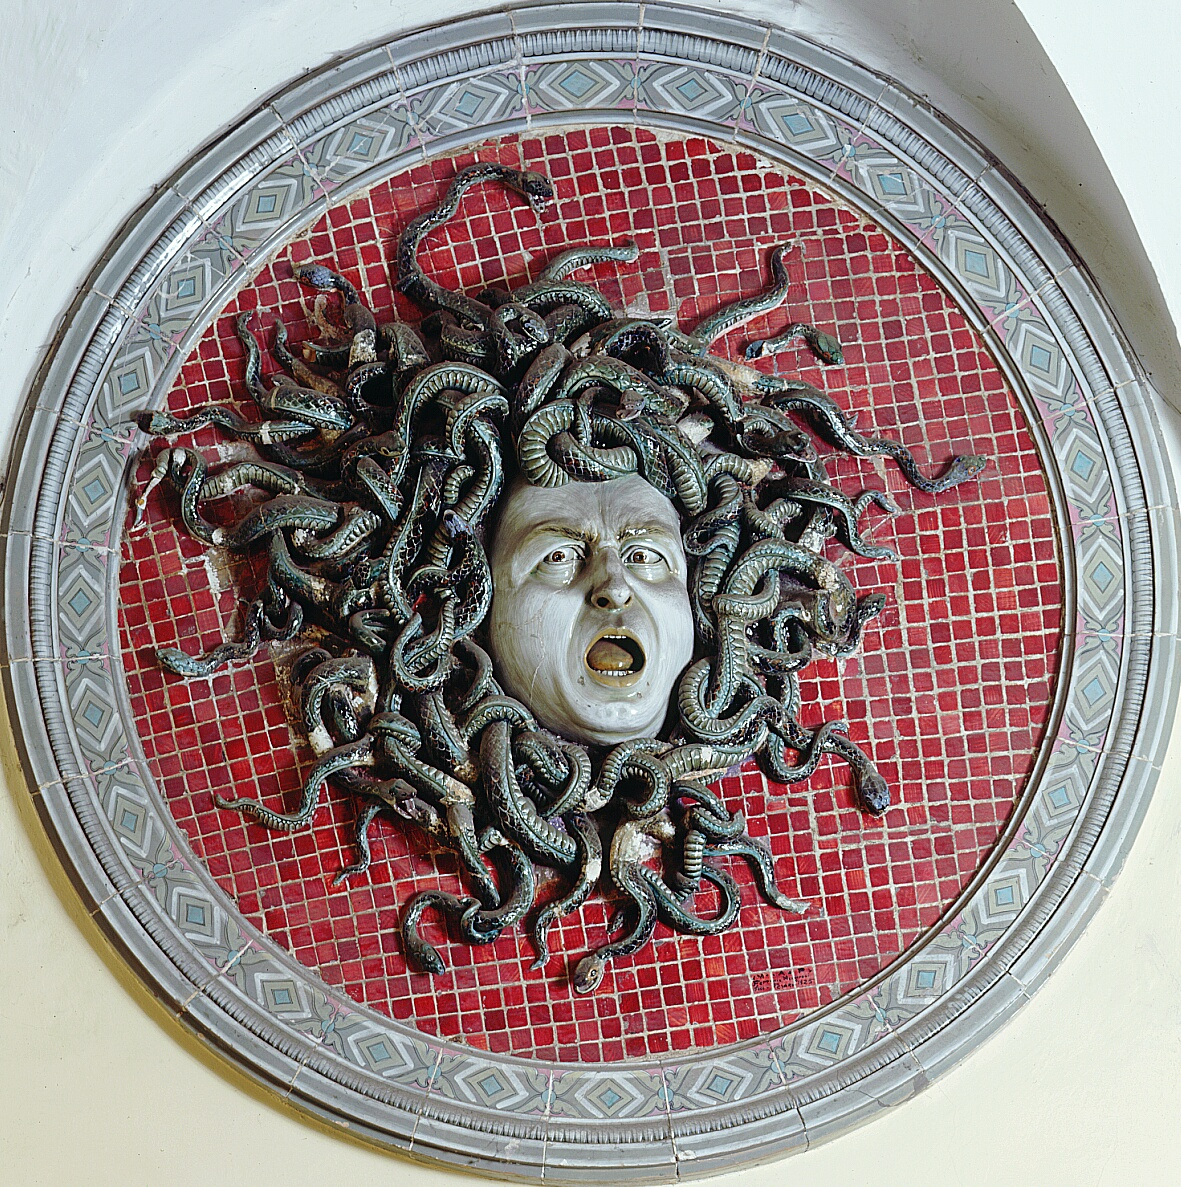
\includegraphics[scale=3.6]{Mengaroni_Ferruccio-Medusa.jpg}
				};
				\jigsaw{6}{4}
			\end{tikzpicture}
		
		\end{minipage}
	
	\end{adjustwidth}
\end{document}